\section{Evaluation}

We evaluated \name using the big data benchmark -- BigBench (BB) \cite{bbench}. We ran experiments on a 40-server CloudLab cluster. We setup Tez atop YARN for the experiment.
\begin{figure}[!h]
	\centering
	\subfloat[Avg. compl. of \burstq jobs]{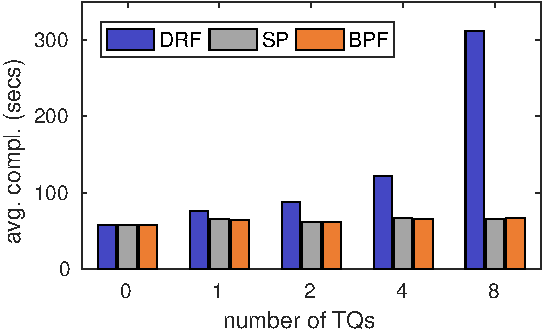
\includegraphics[width=0.47\linewidth]{fig/busty_perf_grt_BB} \label{fig:busty_perf_grt}} 	
	\subfloat[Avg. compl. of \batchq jobs]{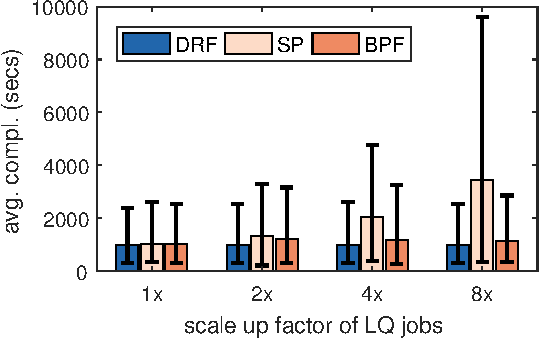
\includegraphics[width=0.47\linewidth]{fig/batch_perf_protect_BB} \label{fig:protecting_batch_jobs}}
	\vspace{-0.15in}	
	\caption{\name can closely approximate the \burstq performance of Strict Priority and the long-term fairness for {\batchq}s of DRF.}
\end{figure}

We compare {\name} to two baseline policies: Strict Priority (SP) \cite{strict_priority} and DRF~\cite{drf}. While SP prioritizes \burstq whenever possible, DRF ensures instantaneous fairness. 


%We focus on what happens when there are more than one \batchq 
In Figure (\ref{fig:busty_perf_grt}), there are a single \burstq and multiple {\batchq}s.
When there are no TQs, the average completion times of \burstq jobs across three schedulers are the same (57 seconds).
As the number of {\batchq}s increases, the performance of DRF significantly degrades because DRF tends to allocate less resource to {\burstq} jobs. 
In contrast, \name and SP give the highest priority to {\burstq}s and the average completion times of \burstq jobs are almost unchanged (65 seconds).

When we have too many {\burstq} jobs, Figure (\ref{fig:protecting_batch_jobs}) highlights that SP allocates too much resource to \burstq jobs that significantly hurts \batchq jobs, while DRF maintains similar average completion times of \batchq jobs. \name performs closely to DRF.

In summary, \name speeds up latency-sensitive jobs by $4.66\times$ compared to DRF, while still maintaining long-term fairness. In the meantime, \name improves the average completion times of throughput-sensitive jobs by up to $3.05\times$ compared to Strict Priority.
%More results can be found in \cite{tech_report}.

Figure \ref{fig:admission_control_cluster} illustrates the admission in the case of multiple {\burstq}s. {\burstq}-0 arrives and receives the performance guarantee. {\burstq}-1 conflicts with {\burstq}-0 and is put into soft-guarantee. {\burstq}-2 is treated like {\batchq}-0 because it requires too much resource.

\begin{figure}[!h]
	\centering
	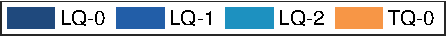
\includegraphics[width=0.6\linewidth]{fig/b1i3_res_usage_legend} 	
	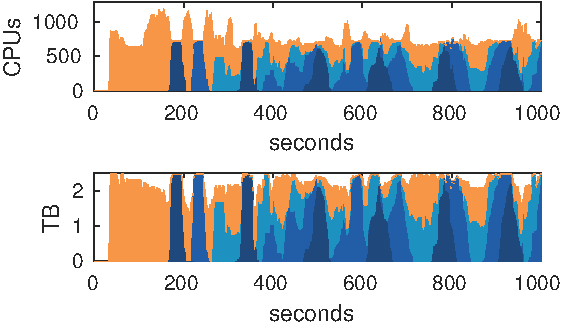
\includegraphics[width=0.8\linewidth]{fig/res_usage_b1i3_BPF_BB} \label{fig:admission_speedfair_cluster}
	\vspace{-0.15in}		
	\caption{[Cluster] \name gives the best performance to \burstq-0, near optimal performance for \burstq-1, and maintains fairness among 4 queues.}
	\label{fig:admission_control_cluster}
\end{figure}

\phantomsection
\label{EndOfPaper}